% ++++++++++++ Controller PSoC Master klassen ++++++++++++++
\subsubsection{Boundary-klasse: Psoc}

\begin{figure}[h]
\centering
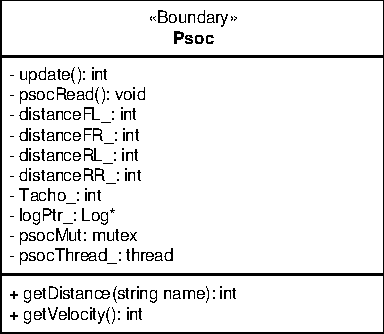
\includegraphics[]{../fig/diagrammer/bil/cd_psoc.pdf}
\caption{Klassebeskrivelse af boundary-klassen Psoc}
\label{fig:cd_psoc}

\end{figure}

\textbf{Attributter}

\begin{table}[h]
	\begin{tabularx}{\textwidth}{| Z | Z | L{10cm} |} \hline
	Navn & Type & Beskrivelse \\\hline
	\texttt{distanceFL\_}  & \texttt{int} 	& Midlertidig variabel der indeholder afstanden fra forreste venstre afstandssensor					\\\hline
	\texttt{distanceFR\_}  & \texttt{int} 	& Midlertidig variabel der indeholder afstanden fra forreste højre afstandssensor					\\\hline
	\texttt{distanceRL\_}  & \texttt{int} 	& Midlertidig variabel der indeholder afstanden fra bagerste venstre afstandssensor					\\\hline
	\texttt{distanceRR\_}  & \texttt{int} 	& Midlertidig variabel der indeholder hastigheden fra Tachometeret									\\\hline
	\texttt{logPtr} 	 & \texttt{Log*} 	& Pointer til Log-klassen, benyttes til at skrive i loggen											\\\hline
	\texttt{psocMut} 	 & \texttt{mutex} 	& Mutex der benyttes til at låse de midlertidige variabler imens der skrives/læses til/fra dem		\\\hline
	\texttt{psocThread\_} & \texttt{thread} 	& Mutex der benyttes til at låse de midlertidige variabler imens der skrives/læses til/fra dem	\\\hline
	\end{tabularx}
	\caption{Attributter for klassen Psoc}
	\label{table:attr_Psoc}
\end{table}
\clearpage

\textbf{Metoder}

\begin{table}[h]
	\begin{tabularx}{\textwidth}{| L{2.5 cm} | Z |} \hline
	Prototype 	& \texttt{int getDistance(string name)} \\\hline
	Parametre 	& \texttt{name} \newline Navnet på den sensor der skal læses fra. Kan rumme én af fire muligheder "FL", "FR", "RL" og "RR". \\\hline
	Returværdi 	& \texttt{int} \newline Seneste afstandsmåling for den pågældende sensor. Værdien er angivet i cm. \\\hline
	Beskrivelse & Metoden læser afstanden som en given sensor befinder sig fra en forhindring. \\\hline
	\end{tabularx}
	\caption{Metodebeskrivelse for \texttt{getDistance}}
	\label{table:met_getdistance}
\end{table}

\begin{table}[h]
	\begin{tabularx}{\textwidth}{| L{2.5 cm} | Z |} \hline
	Prototype 	& \texttt{int getVelocity()} \\\hline
	Parametre 	& \texttt{void} \newline Funktionen tager ingen parametre \\\hline
	Returværdi 	& \texttt{int} \newline Seneste hastighedsmåling for tachometeret. Værdien er angivet i km/t * 10. \\\hline
	Beskrivelse & Metoden læser hastigheden fra tachometeret. \\\hline
	\end{tabularx}
	\caption{Metodebeskrivelse for \texttt{getVelocity}}
	\label{table:met_velocity}
\end{table}
\clearpage